\documentclass[technote]{IEEEtran}
\usepackage{cite}
\usepackage{lipsum}
\usepackage{todonotes}
\usepackage[utf8]{inputenc}
\usepackage{hyperref}
\setlength{\marginparwidth}{1.3cm}

\begin{document}

\title{A Hybrid Approach to Prefetching Based on a Global History Buffer\\ TDT4260 - Computer Architecture}

\author{
  \IEEEauthorblockN{
    Øyvind Robertsen,
    Jonatan Lund,
    Truls Rustad Fossum and
    Katrine Roland
  }

  \IEEEauthorblockA{
    Department of Computer and Information Science\\
    Faculty of Information Technology, Mathematics and Electrical Engineering\\
    Norwegian University of Science and Technology\\
    NTNU, 7491 Trondheim\\
    Norway
  }
}

\maketitle

\begin{abstract}
The abstract goes here.
\end{abstract}

\listoftodos
\section{Introduction}
\label{sec:introduction}

In modern computer architecture, the memory hierarchy plays an important part.
Without intelligent usage of caches and scheduling of requests to main memory, the processor will spend an undesirable amount of time idle while waiting for data.
Prefetching aims to reduce cache misses and increase data availability by attempting to predict which data will be needed in the future and fetch it early. \todo{rephrase}
Designing a prefetcher that performs well for all programs is difficult.
Depending on the type of program, different memory access patterns arise, making it necessary for the prefetcher to be adaptive.

In this paper, we present a prefetcher design that measurably increases performance for a wide range of program types.

Our final prefetcher is an implementation of global history buffer with delta correlation.
The memory accesses made by the instructions are stored in a linked list.
When an instruction is encountered again, the linked list is traversed and the deltas between the earlier accesses are examined to see wether a pair of deltas equal to the most recent ones exist.
If it does, a block is prefetched using the same delta.

This paper provides background (section~\ref{sec:background}) on various prefetcher strategies as well as an overview of our process and methodology (section~\ref{sec:methodology}).
Subsequently, the finished prefetcher design is presented (section~\ref{sec:prefetcher}), followed by results and perfomance details (section~\ref{sec:results}).
Finally, we discuss (section~\ref{sec:discussion}) our findings, provide an overview of some related works (section~\ref{sec:related-work}) and a conclusion (section~\ref{sec:conclusion}).
\todo{better way of writing this?}

%The introduction section introduces the larger research area
%the paper is a part of and illustrates the concrete problem(s) at
%hand the paper tries to solve. It explains the proposed solution
%from a 20.000 feet abstraction level. Furthermore, it states
%the contributions of the paper and briefly highlights its main
%results. It finishes with an outline of the paper, giving a short
%explanation of the contribution/meaning of each section.

\section{Background}
\label{sec:background}
\subsection{Prefetchers}
%The background section covers knowledge that is necessary
%for understanding the proposed solution, but you cannot expect
%the audience of the paper to be familiar with. This is commonly
%the case when you propose solutions that incorporate
%knowledge from different research areas. An example would
%be an implementation of a compression scheme between
%memory and processor in order to decrease memory bandwidth
%utilization. It is very likely that you would need to explain
%the compression scheme, since most computer architecture
%researchers would not be familiar with it.

% == This stuff can probably be assumed known ==
%The speed of processors have been improving much faster than the
%speed of memory and thus memory is not able to keep up with the
%processors. Processors have to wait for too long if needed data
%must be fetched from memory. Caches that are smaller, but faster
%than main memory are thus used to store data which is in use by
%the processor. As the cache needs to be a lot faster than main
%memory, it has to be small to not be too expensive. Therefore it
%is limited what can be stored in the cache

With a simple cache, data is not fetched in to the cache before the
processor needs the data or data in the same block. These misses
are not possible to avoid without fetching blocks before the
processor needs them (prefetching). There are many strategies
available for deciding what to prefetch.

\subsubsection{Sequential prefetching}

The simplest for of prefetching is to just prefetch the next block
as well when fetching a block the processor needs. This can
sometimes be improved on by changing the prefetch distance (instead
of prefetching the next block, prefetch the second or a later one).
Sometimes the processor will need the next block before it is in
the cache even if it was prefetched. In these cases prefetching a
later block can improve performance.

In addition, more than one block can be prefetched (increasing the
prefetch degree). If the running program uses a lot of sequential
memory this can improve performance. If too many blocks are
prefetched, blocks that are still in use can be evicted from the
cache, which can degrade performance.

\subsubsection{Stride Directed Prefetching}

With stride directed prefetching (SDP), the memory address an instruction
accesses is stored together with the program counter address of the instruction
and a valid bit is set. When an instruction is encountered again, the stride
between the address accessed the last time, and the address accessed the
current time is calculated. Then this stride is added to the address currently
being accessed and the block containing the current address is prefetched.

\subsubsection{Reference Prediction Tables}

The reference prediction (RPT) method is similar to SDP, but in
addition stores the stride and a state. The first time an
instruction is encountered, the address is stored as in SDP, and
in addition an initial state is set. The second time an instruction
is encountered, the stride is calculated is in SDP and it is stored.
The state changes to training. The next time the instruction is
encountered, the stride is calculated again, and compared to the
currently stored stride. If they are equal, the state changes to
prefetching and the stride added to the current address is
prefetched.

\subsubsection{Global History Buffer}

With a global history buffer (GHB), all the accesses by the same
instructions are stored in a linked list. When the same
instruction is encountered again, this list is traversed and the
deltas between the addresses accessed are stored. Then the delta
history is searched to see if a pair equal to the most recent pair
of deltas exists. If such a pair is found, the next delta (or
several of the next deltas) is added to the current address,
and the result is prefetched.

\subsection{SPEC CPU2000}
CPU2000 was designed to provide a way to measure performance across
a wide range of hardware. The benchmarks are based on real user
applications. They measure the performance of the processor, memory
and the compiler. CPU2000 contains 25 different benchmarks and
measures both integer and floating point performance.
\cite {bib:cpu2000}

\subsection{M5 simulator}
M5 is an open-source hardware simulation system. It supports multiple
different CPU architectures, one of them being Alpha, which we used.
It has an event-driven memory system which among other features supports
flexible arrangements of the components so it is possible to model
multilevel caches. M5 uses a trace-based CPU model to achieve fast and
accurate measuring of the performance of the memory system.
\cite{bib:m5}


\todo{Different performance measures (accuracy, coverage)}
\todo{Aggressiveness}

\section{Methodology}
\label{sec:methodology}
% \subsection{Description}
% The methodology section explains your experimental setup.
% It should state every bit of information that is necessary in
% order to be able to reproduce your results. It further covers
% your actions taken in order to ensure that you are really
% measuring what you think you are measuring as well as your
% actions that were taken in order to validate your results. The
% goals are to set up realistic experiments and be absolutely
% convinced that you took care of all side-effects as well as to
% state enough information such that your experiments are fully
% reproducible.

\subsection{Simulated Architecture}

We use the M5 computer architecture simulator~\cite{bib:m5} to evaluate different prefetching techniques.
The simulated architecture is that of the Alpha 21264\cite{bib:alpha-21264}, a superscalar, out-of-order CPU.
The simulator is configured with a two level cache system; level 1 is a split cache with 32 kB for instructions and 64 kB for data, level 2 a combined cache of 1 MB.
Access to main memory takes $30$ns over a $64$ bit memory bus clocked at $400$ MHz.

We implement a prefetcher as a set of C++ functions specified by the memory interface of the simulator~\cite[Section 3.2]{bib:doc}.
\texttt{prefetch\_init()}, which is called when the simulation starts, allows us to initialize data structures.
\texttt{prefetch\_access()} is called every time the L2 cache is accessed.
Here, we decide if and what we should prefetch.

The prefetcher is compiled into the simulator before running benchmarks to evaluate its performance.

\subsection{Benchmarking}

The SPEC CPU2000\cite{bib:cpu2000} is a suite of benchmark programs designed to test hardware performance.
To evaluate prefetcher performance, we use a subset of the programs available in the suite.
They are as follows; \texttt{bzip2}, a compression algorithm, \texttt{twolf},
a place-and-route package used in microchip design, \texttt{wupwise}, a solver for a set of
equations in the field of quantum chromodynamics, \texttt{swim} a weather prediction program,
\texttt{applu} and \texttt{ammp}, differential equation solvers, \texttt{galgel}, a solver for a
particular problem in fluid dynamics and \texttt{apsi}, a program used to predict spread of air pollution.

The goal we set for our prefetcher was to achieve as high average speedup as we could, while having no individual benchmark with a speedup of less than $0.95$.
A prefetcher with a negative impact greater than that on one or more types of programs, would be infeasible to use in a real world scenario.
In order to determine whether the goal had been reached, a method of evaluating the developed prefetchers was required.
During this project, the evaluation was done using the M5 computer architecture simulator running a reduced SPEC CPU2000 benchmark suite compiled for an ALPHA architecture.
The simulator was configured with a two level cache system; level 1 was a split cache with 32 kB for instructions and 64 kB for data, level 2 a combined cache of 1 MB.
The prefetchers were implemented in C and compiled into the simulator before running the benchmarks.

After running the benchmarks, the simulator output the speedup, accuracy and coverage the prefetcher had for every benchmark, as well as the number of prefetches identified,
number of prefetches issued and the total number of L2 cache misses for each benchmark. In addition the average speedup (calculated by harmonic mean) of all the benchmarks
was output. We used the average speedup and to some extent the speedup for each benchmark to judge and compare the prefetchers.

Several classical prefetchers were implemented, tested and evaluated to provide a solid starting point.
The implemented prefetchers were a sequential prefetcher, SDP, RPT, and a GHB with delta correlation.

Next, the GHB implementation was extended to also include RTP and ultimately SPD as fall backs whenever the delta correlation did not result in any prefetches being performed.

When testing each prefetcher, the relevant aggressiveness was adjusted (within reasonable limits) for best average speedup.

\subsection{SPEC CPU2000}
CPU2000 was designed to provide a way to measure performance across
a wide range of hardware. The benchmarks are based on real user
applications. They measure the performance of the processor, memory
and the compiler. CPU2000 contains 25 different benchmarks and
measures both integer and floating point performance.

\cite{bib:cpu2000}

\subsection{M5 simulator}
M5 is an open-source hardware simulation system. It supports multiple
different CPU architectures, one of them being Alpha, which we used.
It has an event-driven memory system which among other features supports
flexible arrangements of the components so it is possible to model
multilevel caches. M5 uses a trace-based CPU model to achieve fast and
accurate measuring of the performance of the memory system.

\cite{bib:m5}

\section{Prefetcher (maybe change this title)}
\label{sec:prefetcher}
\subsection{Description}
% This section explains your proposed solution in full detail.
% It needs to strike a fine balance between unnecessary implementation
% details and a level of abstraction that is too high.
% The goal is to give enough detail such that the audience of
% your paper is able to reimplement your scheme, but not more.
% Informative figures and examples are a very powerful tool for
% conveying necessary information to your audience, and are
% often worth more than a thousand words.

The final prefetcher implemented during this project keeps a history of the
previous memory requests issued and uses three different algorithms in a
prioritized order to determine which addresses to prefetch.
An overview of this can be found in Figure \ref{fig:prefetcher}.

\begin{figure*}[h]
	\centering
	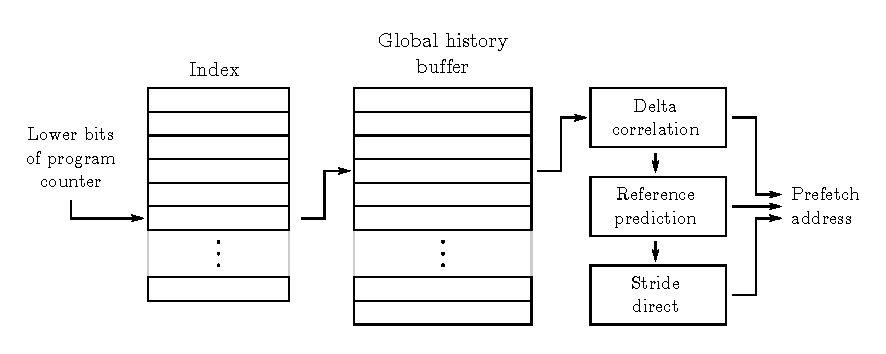
\includegraphics{images/prefetcher.pdf}
	\caption{
		Basic structure and data flow in prefetcher. The lower bits of the
		program counter at the load instruction is used to look up the first
		entry of a history chain in the global history buffer. Next, the history
		is used to determine which addresses to prefetch using one of the
		algorithms on the right.
	}
	\label{fig:prefetcher}
\end{figure*}

The history tracking is implemented using a global history buffer and an index.
Given an instruction address, the lower bits can be used to look up an entry in
the global history buffer through the index.
This entry is the first in a doubly linked list of memory addresses accessed by
instructions with matching lower bits in their addresses.

On a memory request, the index and global history buffer is updated and the
linked list of addresses is used to calculate a history of deltas, the
differences between consecutive memory addresses in the list.
This list is passed on to the algorithms used to determine which addresses to
prefetch.

First in line is the delta correlation algorithm.
It searches the history for the two most recent deltas.
If found, we assume to have found a loop of deltas and issue prefetches for the
addresses following the current with the deltas from the history.
In the cases where the degree is higher than the length of the matching history,
the process is repeated from the last memory address prefetched until enough
prefetches have been issued.
This strategy fails to produce prefetches when

\begin{enumerate}
	\item the history contains less than 3 entries for the given program
		counter or
	\item the two most recent deltas do not appear anywhere earlier in the
		history.
\end{enumerate}

Should the delta correlation fail to produce prefetches, the delta history is
handed on to an algorithm inspired by the reference prediction table.
The prefetches are issued using the most recent delta in the history if the two
last entries are equal.
In this case, the same delta is simply added to the memory address requested
several times to produce all prefetch addresses.

In the cases where the history contains one, and only one delta, the prefetcher
uses this delta to issue prefetches as for the previous algorithm.
This is equivalent to what a stride direct prefetcher would do.

It is important to note that both the index and the global history buffer is
limited in size. For the history buffer, this is handled by overwriting the
oldest entry. For the index, only the lower bits of the instruction address is
used, thus we may experience collisions.

%TODO: Can we assume there to be a low number of collisions based on the results
%      from associative caches in Computer Architecture: A Quantitative Approach?

\section{Results and Discussion}
\label{sec:results-and-discussion}
% \subsection{Description}
% This section presents the results of your experiments,
% comparing your solution to other schemes. The metrics of
% interest are highly dependent on the topic of research, but
% should optimally cover all interesting aspects of your scheme.
% Informative graphs or tables are the key to a good result
% section.
% Furthermore, you need to discuss your results. You should
% give explanations of distinctive points and outliers in your
% results. It is also necessary to state why your scheme is
% better/worse compared to the other schemes. Thus, this section
% consists of two parts: the results of your experiments, as well
% as an explanation as to why the results are as they are

The speedup associated with each prefetcher for each benchmark, as
well as the average speedup across benchmarks calculated by harmonic
mean, is shown in Figure \ref{fig:comparison}. We test with
prefetching degree varying from $1$ to $7$. For each prefetcher,
numbers for the plot are taken from the degree yielding the highest
average speedup.

The \texttt{ammp} benchmark is noticably more sensitive to different
prefetching strategies than the rest. This indicates that relative to
the other benchmarks, \texttt{ammp} spends more time in code for which
it is easy to make good prefetching predictions.

\texttt{ammp} and \texttt{wupwise} are the two benchmarks with the
highest speedup.  For the rest, speedup is $1.00\pm0.10$. To better
understand why this is, we look at the accuracy and coverage of the
various prefetchers in Figures \ref{fig:accuracy} and
\ref{fig:coverage}. For most of the benchmarks with low
speedup, either accuracy is low, coverage is low or a combination of
both.

We see that our hybrid prefetcher has lower average speedup than the
simple DC implementation.  By comparing the results in greater detail,
we try to understand why.

\begin{figure*}
  \centering
  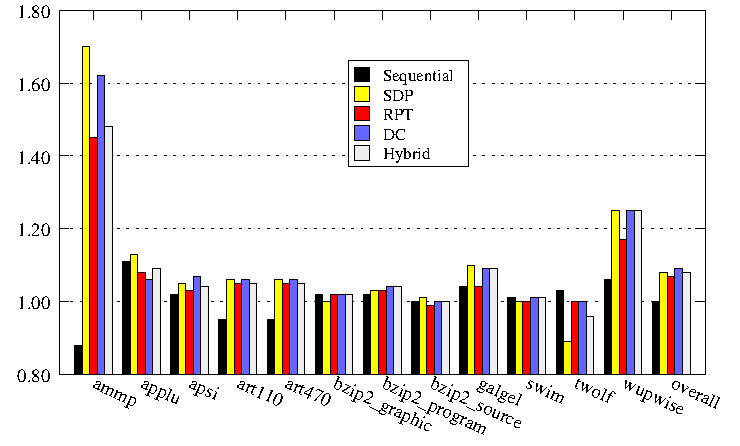
\includegraphics{plots/overview_speedup.pdf}
  \caption{
    Speedup as measured during simulation for each prefetcher grouped by
    benchmark.
    The degree for each prefetcher has been selected to maximize the overall
    performance as measured by the harmonic average displayed to the right.
  }
  \label{fig:comparison}
\end{figure*}

\begin{figure*}
  \centering
  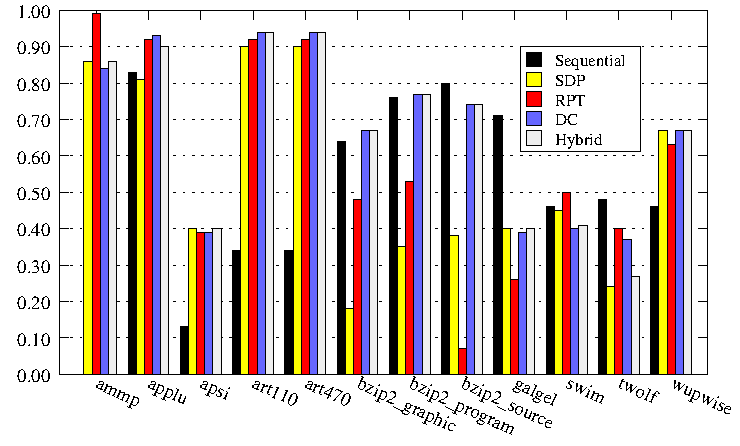
\includegraphics{plots/accuracy_overview.pdf}
  \caption{
      Comparison of prefetcher accuracy for all benchmarks.
      The degrees have been chosen to maximize the harmonic average speedup.
  }
  \label{fig:accuracy}
\end{figure*}

\begin{figure*}
  \centering
  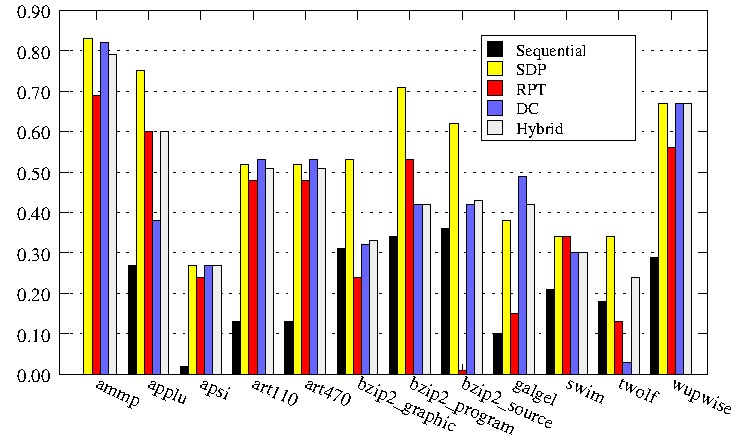
\includegraphics{plots/coverage_overview.pdf}
  \caption{
      Comparison of prefetcher coverage for all benchmarks.
      The degrees have been chosen to maximize the harmonic average speedup.
  }
  \label{fig:coverage}
\end{figure*}


An interesting example of how the different prefetchers differ, is the
\texttt{ammp} benchmark.  This is the benchmark where the sequential
prefetcher performs worst; it degrades performance significantly and a
higher prefetching degree only makes it worse.  For degree 1, it has
an extremely low accuracy of only $0.1\%$ which means most of the
effort put into prefetching blocks is wasted.

The SDP prefetcher on the other hand performs quite well and gives a speedup of
$1.7$ for a prefetching degree of $3$. For this degree, an accuracy of $86\%$
means much fewer of the prefetches are wasted effort.  As the only difference
between this and the sequential prefetcher is the variable stride used for SDP,
this indicates that the \texttt{ammp} benchmark accesses memory in a linear,
but strided fashion.

The remaining prefetchers all handle strided access and results comparable with
SDP should therefore be expected.  For delta correlation, the best results are
achieved with a prefetching degree of $6$.  At this degree, $84\%$ of the
prefetches turn out to be useful.  The fetches for useless data is probably
what makes delta correlation less effective than SDP despite the improved
coverage.
%TODO: Comment how many of these were already in MSHRs?
This is also suggested by the $44\%$ increase in average cache miss latency.

For the hybrid prefetcher developed during this project, the speedup on \texttt{ammp} is slightly
worse than for the pure delta correlation approach.
Despite falling back to RPT and eventually SDP, the hybrid approach identifies
fewer prefetches than the delta correlating prefetcher.
Combined with about the same accuracy as for delta correlation, this can explain
the reduced performance.
\todo{Why? It should have more}

Another interesting benchmark is \texttt{wupwise}.
In this benchmark, SDP, delta correlating and hybrid prefetchers all give a
consistent speedup of $1.25$ for all the degrees tested.
RPT is also giving a very consistent speedup of around $1.21$, which is sightly
worse than sequential for degrees greater than 1.
This can be explained if the benchmarks contains long runs of strided memory
access.
Thus the first block after the requested one may not be needed, as assumed in
sequential prefetching, but the next one may be.
As a result, sequential prefetching with a higher degree performs better up to a
certain limit at the maximum stride observed.

Comparing SDP and RPT, both stride based, it becomes clear that the lower
performance of RPT can be explained by a combination of a slightly lower
accuracy and a lower number of identified prefetches.
This may be due to RPT, being more restrictive, only identifies prefetches when
the two last deltas are equal, in contrast to SDP which only requires one.
On the other hand, delta correlation still maintains the same performance while
requiring even more history.
A possible explanation may be that the benchmark's memory access pattern
includes a lot of repeating patterns exploitable by delta correlation.
If the patterns also include some runs of equal deltas, this should be
beneficial to SDP as well because it utilizes shorter runs of equal deltas
better than RPT.

This may also be the reason for the good performance of sequential prefetching
compared to RPT.
From the statistics, RPT only identifies about $72\%$ the number of prefetches
sequential does.
Despite the lower accuracy, this results in a coverage about $15\%$ higher for
sequential.

A noteworthy observation is that the hybrid prefetcher performs comparably to
SDP and delta correlation, even though it follows the RPT policy when there are
only two history entries.
This is natural since delta correlation is always used when possible, otherwise
SDP provides adequate prediction and the few predictions made using RPT does not
affect the overall performance.

The only benchmark where the hybrid prefetcher performs notably worse than the
delta correlating prefetcher is the \texttt{twolf} benchmark.
Comparing the number of identified prefetches, the hybrid prefetcher identifies
about $10$ times as many as the delta correlating prefetcher.
These prefetches do not turn out to be beneficial in most cases as can be seen
from the lower accuracy of the hybrid prefetcher.

Since the hybrid approach uses the same strategy as SDP and RPT when too little
history is available for delta correlation, poor performance for RPT and SDP is
also to be expected.
This proves to be the case as well; the SDP prefetcher has the absolutely worst
performance.
Even though it identifies almost the same number of prefetches as the much
better performing RPT, it falls short on accuracy.

An example where the hybrid prefetcher actually performs better than the delta
correlating prefetcher can be found by looking at the \texttt{applu} benchmark.
This happens for degrees ranging from $1$ to $4$, which is due to a higher
number of identified prefetches by the hybrid implementation while both
prefetches maintain an accuracy above $90\%$.

Furthermore, we have an example of the sequential prefetcher performing much
better than all the stride based prefetchers for all degrees above 1.
This may be due to very irregular strides, causing the stride based prefetchers
to fetch useless blocks, which degrade performance.

\section{Related Work}

\section{Conclusion}
\label{sec:conclusion}
%This section concludes your work by briefly repeating the
%goal of your work and stating the main results. It can also
%include planned future work.

Of the different prefetching strategies explored in this report,
global history buffer with delta correlation has the best average
speedup while no benchmark has a speedup of less than 0.95.

This prefetcher has a higher average speedup than our hybrid
approach. This falsifies our hypothesis that we would achieve
a higher average speedup by falling back on RTP and SDP when
DC does not find anything to prefetch.

However, while this prefetcher has the highest average
speedup, simpler prefetchers are sometimes better on
individual benchmarks, showing that while global history buffer
with delta correlation is on average the best for the benchmarks
used for testing in this case, it is not the best in all cases.

To improve the prefetcher further, a scheme to choose which
entry should be evicted when the global history buffer is full,
based on the probability that the entry will be useful in the
future, could be introduced.

% Improvement: Tag for index table (like in caches) to prevent mixing histories
% from different PCs


\bibliographystyle{plain}
\bibliography{bibliography}

\end{document}
